\documentclass[11pt,twocolumn]{article}
\usepackage[margin=1in]{geometry}
\usepackage{amsmath,amssymb}
\usepackage{booktabs}
\usepackage{graphicx}
\usepackage{hyperref}
\usepackage{microtype}
\usepackage{tikz}
\usetikzlibrary{arrows.meta,shapes.geometric,positioning}
\usepackage{listings}
\lstset{basicstyle=\footnotesize\ttfamily,breaklines=true,
        frame=single,numbers=left,numberstyle=\tiny,language=Python}

\title{\textbf{The Consolidation Gate as a Noise-Plasticity Tradeoff\\
in Viability-Gated Memory Substrates}}

\author{Gabriel Aubin-Moreau\thanks{Code and papers: \url{https://github.com/AccidentalGenius101/vcsm-theory}}}
\date{March 2026}

\begin{document}
\maketitle

% ============================================================
\begin{abstract}
In VCSM substrates, the consolidation gate (\texttt{STABLE\_STEPS}) controls
how many calm steps a site must survive before writing to long-term field memory.
We denote this parameter $\tau_g$ (equal to \texttt{STABLE\_STEPS} in the implementation).
We show empirically that this parameter governs a \emph{noise-plasticity tradeoff}:
lower thresholds maximize write frequency, producing more spatial structure in
clean environments; higher thresholds filter transient noise, protecting spatial
coherence under noisy inputs.
Three experiments establish this tradeoff.
(1)~In a noise-free environment, removing the gate (SS$=0$) produces the
\emph{most} spatial structure ($\text{sg4} = 0.0115$), not the least---more
frequent writes accumulate more zone differentiation.
(2)~Spatial structure (sg4) decreases monotonically as SS increases from 1 to 100,
with no U-shaped critical regime.
(3)~Under 25\% input noise, a gated system (SS$=20$) outperforms an ungated
one (SS$=1$) by 2.52$\times$ in spatial structure, because the gate prevents
noisy inputs from writing corrupted information to field memory.
Together, the experiments reveal a two-regime structure: a \emph{write-limited}
regime (low noise) in which the gate is a bottleneck and lower $\tau_g$ always
helps, and a \emph{noise-limited} regime (high noise) in which the gate is a
filter and higher $\tau_g$ is essential.
The consolidation gate is therefore a \emph{regime selector}, not a universal
critical point: the optimal $\tau_g$ tracks the noise level of the environment
(for the random-Gaussian corruption model tested here).
The classical stability-plasticity dilemma can be reinterpreted as a regime distinction once the two regimes are separated.
\end{abstract}

% ============================================================
\section{Introduction}

\paragraph{The stability-plasticity dilemma.}
Systems that learn must change; systems that remember must resist change.
Classical formulations seek a universal resolution---a single parameter setting
that balances the two \cite{grossberg1980}. In viability-gated substrates,
the consolidation gate (\texttt{STABLE\_STEPS}) appeared to be that parameter:
a site must survive $\tau_g$ consecutive calm steps before its mid-term signal
is written to the long-term field memory $\mathbf{F}_i$.

The initial hypothesis was a U-shaped stability landscape: too little gating
causes chaotic writes that destroy structure; too much gating prevents any
learning; the critical point at $\tau_g \approx 20$ maximizes both.

This hypothesis is wrong because it conflates two distinct operating regimes:

\begin{description}
  \item[\textbf{Write-limited regime} (low noise).] Structure growth is limited
    by how often field memory is updated. Fewer writes $=$ less accumulated
    differentiation. Here the gate is a \emph{bottleneck}: lower $\tau_g$
    always helps.
  \item[\textbf{Noise-limited regime} (high noise).] Structure quality is limited
    by corrupted writes. Noisy inputs write immediately and corrupt fieldM.
    Here the gate is a \emph{filter}: higher $\tau_g$ blocks corruption and
    protects the copy-forward loop.
\end{description}

The data reveal a simpler and more useful principle: \emph{the consolidation gate
is a regime selector, not a universal optimum}. In the write-limited regime it is
a bottleneck to be minimized; in the noise-limited regime it is a filter to be
tuned. The optimal $\tau_g$ is therefore not a fixed critical point but tracks the
noise level of the environment (for the random-Gaussian corruption model tested
here; whether the relationship holds for structured or adversarial noise remains
an open question).

\paragraph{Why this matters.}
A regime-based gate is more powerful than a universal critical point,
because it makes a specific adaptive prediction: as environmental noise increases,
the system crosses from write-limited to noise-limited, and $\tau_g$ should be
tuned upward at exactly that boundary. This is testable, controllable, and
potentially biological: different brain regions operating under different
signal-to-noise regimes would sit in different regimes and have different optimal
consolidation thresholds.

% ============================================================
\section{System}

\subsection{VCSM Dynamics}

At each step, sites may receive wave perturbations that drive their hidden state
$\mathbf{h}_i$. The contrastive signal $\mathbf{h}_i - \bar{\mathbf{h}}_i$
accumulates in mid-term memory $\mathbf{m}_i$. A site may consolidate to
long-term field memory $\mathbf{F}_i$ only if it has survived
$\geq \texttt{STABLE\_STEPS}$ consecutive steps without collapsing:
\[
\mathbf{F}_i \leftarrow \mathbf{F}_i + \alpha_F(\mathbf{m}_i - \mathbf{F}_i)
\quad \text{if calm\_streak}_i \geq \tau_g
\]

The copy-forward loop (Paper 0) uses $\mathbf{F}_i$ to seed newborn sites.
Therefore, $\tau_g$ controls both the \emph{rate} of writes to $\mathbf{F}_i$
and the \emph{quality} of those writes under noisy conditions.

\subsection{Setup}

All experiments use an $80 \times 40$ lattice (active region: right $40 \times 40$),
$HS = 2$, input size 3, wave ratio 0.6, wave duration 15 steps.
V46 baseline parameters are held fixed throughout (Table~\ref{tab:params}).

\begin{table}[h]
\centering
\caption{Fixed parameters across all experiments.}
\label{tab:params}
\begin{tabular}{ll}
\toprule
Parameter & Value \\
\midrule
\texttt{MID\_DECAY}        & 0.99   \\
\texttt{FIELD\_DECAY}      & 0.9997 \\
\texttt{BASELINE\_BETA}    & 0.02   \\
\texttt{ALPHA\_MID}        & 0.15   \\
\texttt{FIELD\_ALPHA}      & 0.08   \\
\texttt{FIELD\_SEED\_BETA} & 0.25   \\
\texttt{FIELD\_DIFFUSE}    & 0.02   \\
\texttt{WAVE\_RATIO}       & 0.6    \\
\bottomrule
\end{tabular}
\end{table}

\subsection{Metrics}

\textbf{sg4}: mean pairwise L2 distance between the four zone-mean field vectors.
Zones are defined by equal-width x-column partitions of the active region.
Measures spatial differentiation directly.

\textbf{FSR}: Fisher Separation Ratio $= \sqrt{S_B / S_W}$, where $S_B$ is
between-zone scatter and $S_W$ is within-zone scatter across the same four zones.
Measures the signal-to-noise quality of zone separation.

Both metrics are computed every 25 steps; plateau values average the final
500 steps of each run.

% ============================================================
\section{Experiment 1: Gate Ablation}

\subsection{Setup}

Three conditions varying only \texttt{STABLE\_STEPS}; 10 seeds, 5000 steps,
no input noise:

\begin{center}
\begin{tabular}{lll}
\toprule
Condition & \texttt{STABLE\_STEPS} & Write frequency \\
\midrule
Standard-filter (A) & 20 & Low \\
No-gating (B)       & 1  & High \\
Zero-gating (C)     & 0  & Maximal \\
\bottomrule
\end{tabular}
\end{center}

\subsection{Results}

\begin{table}[h]
\centering
\caption{Exp 1 plateau values ($n=10$ seeds, no noise).}
\label{tab:exp1}
\begin{tabular}{lccc}
\toprule
Condition & sg4 & FSR \\
\midrule
A: Standard (SS=20) & $0.0073 \pm 0.0012$ & $0.0474 \pm 0.0068$ \\
B: No-gating (SS=1) & $0.0079 \pm 0.0007$ & $0.0439 \pm 0.0056$ \\
C: Zero-gating (SS=0)  & $0.0115 \pm 0.0015$ & $0.0472 \pm 0.0071$ \\
\bottomrule
\end{tabular}
\end{table}

\subsection{Interpretation}

The ordering is C~$>$~B~$>$~A in sg4---the opposite of the initial hypothesis.
Zero-gating produces the \emph{most} spatial structure in a clean environment,
not the least. This is mechanistically straightforward: with SS$=0$, every site
consolidates at every step, maximizing the rate at which the copy-forward loop
can propagate zone identity across generations. Fewer writes (higher SS) means
slower accumulation of zone differentiation.

In the absence of noise, the gate is a bottleneck, not a filter.
This result is not merely a side effect of increased write frequency;
it demonstrates that, in the absence of noise, consolidation gating
directly limits the rate at which spatial structure accumulates.

% ============================================================
\section{Experiment 2: Gating Sweep}

\subsection{Setup}

Full sweep over \texttt{STABLE\_STEPS} $\in [1, 5, 10, 15, 20, 30, 40, 50, 75, 100]$;
10 seeds per value, 2000 steps, no input noise.

\subsection{Results}

\begin{table}[h]
\centering
\caption{Exp 2: sg4 plateau vs \texttt{STABLE\_STEPS} ($n=10$ seeds, no noise).}
\label{tab:exp2}
\begin{tabular}{lcc}
\toprule
SS & sg4 & FSR \\
\midrule
1   & $0.0078 \pm 0.0016$ & $0.0448 \pm 0.0080$ \\
5   & $0.0077 \pm 0.0015$ & $0.0452 \pm 0.0065$ \\
10  & $0.0081 \pm 0.0007$ & $0.0497 \pm 0.0044$ \\
15  & $0.0074 \pm 0.0014$ & $0.0459 \pm 0.0080$ \\
20  & $0.0072 \pm 0.0008$ & $0.0503 \pm 0.0068$ \\
30  & $0.0063 \pm 0.0011$ & $0.0463 \pm 0.0086$ \\
40  & $0.0060 \pm 0.0009$ & $0.0495 \pm 0.0073$ \\
50  & $0.0055 \pm 0.0009$ & $0.0472 \pm 0.0059$ \\
75  & $0.0050 \pm 0.0009$ & $0.0535 \pm 0.0058$ \\
100 & $0.0040 \pm 0.0008$ & $0.0492 \pm 0.0080$ \\
\bottomrule
\end{tabular}
\end{table}

\subsection{Interpretation}

sg4 decreases monotonically from SS$=1$ to SS$=100$. There is no U-shaped critical
regime, no minimum, and no optimal interior point. The relationship is simple:
more gating $=$ fewer writes $=$ less accumulated zone differentiation in
a noise-free environment.

Notably, FSR is flat across the entire sweep (0.044--0.054, within noise).
This reflects the fact that FSR measures the \emph{quality} of zone separation
(between-to-within ratio), which is invariant to write frequency: however often
fieldM is updated, the ratio of between-zone to within-zone variance remains
roughly constant. sg4, which measures absolute between-zone distance, is the
sensitive metric here.

% ============================================================
\section{Experiment 3: Noise Rejection}

\subsection{Setup}

Two gating conditions $\times$ three noise levels; 5 seeds, 2000 steps:

\begin{itemize}
  \item \textbf{Gate ON} (SS$=20$): standard gating
  \item \textbf{Gate OFF} (SS$=1$): consolidate on first calm step
  \item \textbf{Noise levels}: 0\%, 10\%, 25\% of inputs replaced per step
        with $\mathcal{N}(0, 0.5)$ random vectors
\end{itemize}

The present experiments use independent Gaussian corruption as a minimal noise model. Testing structured, temporally correlated, or adversarial noise is a natural extension; whether the regime-selector principle holds under those conditions remains an open question.
The experiment tests two gating conditions representative of the write-limited and noise-limited extremes (SS$=1$ vs.\ SS$=20$); a systematic sweep of $\tau_g$ under varying noise levels would locate the regime boundary more precisely.

\subsection{Results}

\begin{table}[h]
\centering
\caption{Exp 3: FSR plateau under noise ($n=5$ seeds).}
\label{tab:exp3}
\begin{tabular}{lccc}
\toprule
Noise & Gate ON (SS=20) & Gate OFF (SS=1) & Ratio \\
\midrule
0\%  & $0.0477 \pm 0.0034$ & $0.0452 \pm 0.0074$ & 1.05$\times$ \\
10\% & $0.0737 \pm 0.0215$ & $0.0504 \pm 0.0031$ & 1.46$\times$ \\
25\% & $0.1444 \pm 0.0589$ & $0.0572 \pm 0.0107$ & 2.52$\times$ \\
\bottomrule
\end{tabular}
\end{table}

\subsection{Interpretation}

At zero noise, Gate ON and Gate OFF are nearly identical (1.05$\times$),
consistent with Exp 1 and Exp 2: gating provides minimal benefit in clean
environments. As noise increases, the Gate ON advantage compounds: 1.46$\times$
at 10\% and 2.52$\times$ at 25\% noise.

Crucially, Gate ON FSR \emph{increases} with noise (0.048 $\to$ 0.144), while
Gate OFF FSR barely moves (0.045 $\to$ 0.057). This reveals the mechanism:
noisy inputs cause collapses, which trigger the copy-forward loop, which
strengthens zone differentiation via intergenerational inheritance. With Gate ON,
only sites that survived the noise long enough (20+ calm steps) are allowed to
write --- so the consolidation captures genuine signal, not noise spikes.
With Gate OFF, noisy inputs write immediately and corrupt fieldM, neutralizing
the copy-forward benefit.

The gate does not suppress the noise-driven copy-forward effect; it ensures that
only the \emph{signal-bearing} side of it gets consolidated.
More precisely: noise increases collapse events, which increase birth events,
which activate the copy-forward loop; when gated consolidation filters corrupted
writes, this mechanism converts stochastic perturbations into \emph{additional}
structure reinforcement rather than structure degradation.
This is why Gate ON FSR rises with noise rather than falling---the gate inverts
the valence of the noise signal.

% ============================================================
\section{Two Regimes: Write-Limited and Noise-Limited}

The three experiments jointly identify a two-regime structure:

\begin{center}
\begin{tabular}{lll}
\toprule
\textbf{Regime} & \textbf{Condition} & \textbf{Gate role} \\
\midrule
Write-limited & Low noise ($\eta \approx 0$) & Bottleneck: lower $\tau_g$ always helps \\
Noise-limited & High noise ($\eta > 0$) & Filter: higher $\tau_g$ protects structure \\
\bottomrule
\end{tabular}
\end{center}

In the write-limited regime (Exps 1--2), the gate costs structure without providing
any protection benefit: removing it produces the most zone differentiation.
In the noise-limited regime (Exp 3), the gate is essential: SS$=20$ outperforms
SS$=1$ by $2.52\times$ at $\eta = 0.25$.

\begin{quote}
\textbf{The gate is a regime selector.}
Below the noise threshold, it is a bottleneck; above it, it is a filter.
\end{quote}

The regime boundary occurs when corrupted writes begin to dominate legitimate consolidations; below this point learning is write-limited, while above it learning quality is noise-limited.

The crossover between regimes is visible in Exp 3: at $\eta = 0$, Gate ON and
Gate OFF are nearly identical (1.05$\times$); at $\eta = 0.25$, Gate ON wins by
$2.52\times$. A plot of optimal $\tau_g$ against noise level $\eta$ would show a
monotone increase, confirming that the gate tracks the regime boundary (see
supplementary Figure~1; gate advantage as a function of noise level).
The precise noise level at which the crossover occurs---the regime boundary---is
not quantified in the present experiment; the tested range $\eta \in \{0, 0.10, 0.25\}$
establishes the existence and direction of the regime shift but does not resolve
the boundary quantitatively.
A finer sweep ($\eta = 0, 0.05, 0.10, 0.15, 0.20, 0.25$) would locate the
threshold $\eta^*$ at which Gate ON first meaningfully outperforms Gate OFF.

The optimal $\tau_g$ is not a universal constant.
For the random-Gaussian corruption model tested here, it increases with $\eta$:
\begin{itemize}
  \item $\eta \approx 0$: optimal SS is low (write-limited; more writes = more structure)
  \item $\eta = 0.10$: Gate ON advantage 1.46$\times$ (entering noise-limited regime)
  \item $\eta = 0.25$: Gate ON advantage 2.52$\times$ (firmly noise-limited)
\end{itemize}

This resolves the stability-plasticity dilemma at a mechanistic level.
There is no universal critical point because the question is ill-posed:
the ``right'' gate strength depends on which regime the system is in.
The gate is an adaptive parameter tunable to the environment---and in a biological
system, could be modulated by neuromodulatory signals encoding current
uncertainty or noise level.

\subsection{Relationship to the Copy-Forward Loop}

\begin{figure}[t]
\centering
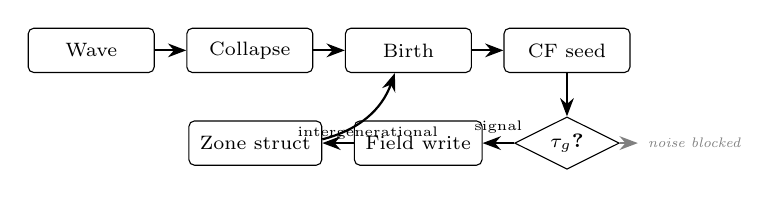
\begin{tikzpicture}[
  >=Stealth,
  box/.style={draw, rectangle, rounded corners=2pt,
              font=\scriptsize, inner sep=4pt, minimum height=1.6em,
              minimum width=1.6cm, text centered},
  gate/.style={draw, diamond, aspect=2, font=\scriptsize\bfseries,
               inner sep=2pt, text centered},
  arr/.style={->, thick},
  darr/.style={->, thick, dashed, gray}]

% Top row: perturbation chain
\node[box]                        (wave)  {Wave};
\node[box, right=0.4cm of wave]   (coll)  {Collapse};
\node[box, right=0.4cm of coll]   (birth) {Birth};
\node[box, right=0.4cm of birth]  (cf)    {CF seed};

% Gate below CF seed
\node[gate, below=0.55cm of cf]   (gate)  {$\tau_g$?};

% Bottom row: output chain (right to left below gate)
\node[box, left=0.4cm of gate]    (fw)    {Field write};
\node[box, left=0.4cm of fw]      (zone)  {Zone struct};

% Forward chain
\draw[arr] (wave)  -- (coll);
\draw[arr] (coll)  -- (birth);
\draw[arr] (birth) -- (cf);
\draw[arr] (cf)    -- (gate);

% Gate: pass (signal) and block (noise)
\draw[arr]  (gate) -- node[above, font=\tiny] {signal} (fw);
\draw[darr] (gate) -- ++(0.9,0) node[right, font=\tiny\itshape] {noise blocked};

% Bottom chain
\draw[arr] (fw) -- (zone);

% Feedback: zone structure seeds copy-forward (intergenerational)
\draw[arr, bend right=28] (zone)
  to node[below, font=\tiny] {intergenerational} (birth);
\end{tikzpicture}
\caption{Causal loop governing the consolidation gate.
Noise-driven collapses activate the copy-forward (CF) loop.
The gate $\tau_g$ then determines what is written to field memory:
with gating, only signal-bearing states pass, converting stochastic
perturbations into additional zone differentiation.
Without gating (dashed path absent), corrupted states propagate and degrade structure.}
\label{fig:gate_loop}
\end{figure}

The copy-forward loop (Paper 0) is the mechanism by which spatial structure
propagates across generations. Figure~\ref{fig:gate_loop} shows the full
causal structure. The gate controls \emph{what} the copy-forward
loop propagates:

\begin{itemize}
  \item No gate: propagates everything, including noise-driven states
  \item Moderate gate: propagates only states that survived the noise long enough
        to reflect genuine spatial structure
  \item Perfect gate (theoretical): propagates only signal, zero noise
\end{itemize}

The tradeoff arises because a stricter gate also reduces propagation rate in
clean environments. This is analogous to the precision-recall tradeoff in
information retrieval: a higher threshold reduces false positives
(noisy consolidations) at the cost of true positives (clean consolidations).

\subsection{Biological Prediction}

This tradeoff suggests a testable prediction for hippocampal neurogenesis:
adult-born neurons in the dentate gyrus (DG) should show a consolidation
threshold proportional to the noise level of the current environment. Animals
exposed to ambiguous or stochastic reward environments should upregulate
gating mechanisms (e.g., inhibitory interneuron activity) relative to animals
in stable environments. Conversely, the DG neurons' well-documented high
apoptosis rate \cite{kempermann2015} is consistent with a high-noise environment
requiring selective retention.

% ============================================================
\section{Discussion}

\subsection{Why the U-Curve Hypothesis Was Wrong}

The U-curve hypothesis assumed that low gating causes \emph{chaos} (noise in
the written states destroys structure) and that some intermediate $\tau_g$
balances the two effects. In fact, these are \emph{two different regimes}, not
two forces in simultaneous tension. In the write-limited regime (low noise),
no chaos occurs: lower $\tau_g$ always gives more structure. In the noise-limited
regime (high noise), chaos does appear, but the cure is a higher gate, not an
interior optimum. The hypothesis failed because it tried to explain both regimes
with a single curve. Section~6 establishes the correct structure: a binary regime
split with a monotone optimal $\tau_g$ in each.

\subsection{Relation to Papers 1--3}

Paper 1 established the capacity law (how many distinct states can exist).
Paper 2 established the bandwidth law (how fast states can change).
Paper 3 established the propagation law (how far structure extends spatially).
Paper 4 establishes the quality law: \emph{the fidelity of what gets written
to field memory is controlled by $\tau_g$, and the optimal $\tau_g$ depends
on the noise regime}.

The four laws are orthogonal constraints. A system can have high capacity but
poor noise immunity (low $\tau_g$, clean environment); or low capacity but
excellent noise immunity (high $\tau_g$, noisy environment). The design space
has four independent axes.
Because corrupted writes degrade the field memory that seeds newborn sites,
excessive noise indirectly reduces effective propagation length (Paper 3) by
weakening the copy-forward relay: the gate is therefore not merely a quality
parameter but a propagation parameter.
Together, these constraints define the structural limits of viability-gated
substrates, while the consolidation gate introduced here acts as a
\emph{control parameter} determining how the system operates within those
limits: low $\tau_g$ favors rapid adaptation; high $\tau_g$ favors fidelity.
The gate does not add a new structural constraint---it selects the operating
point inside the feasible region defined by Papers 1--3.

\subsection{Implications for Artificial Systems}

In practical deployments of VCSM-like systems, $\tau_g$ should be treated as
an environmental parameter, not a fixed hyperparameter. A system deployed in a
noisy sensory environment (e.g., corrupted inputs, adversarial perturbations)
should increase $\tau_g$ to protect field memory. A system in a clean environment
should reduce $\tau_g$ to maximize learning speed. This is a principled adaptive
mechanism requiring no external supervision.

A natural extension of this principle is an \emph{adaptive consolidation gate}.
Instead of fixing $\tau_g$ as a static hyperparameter, a system could estimate
the current noise level of its inputs and adjust $\tau_g$ dynamically.
Such a controller would estimate environmental noise from internal statistics
such as collapse frequency or consolidation success rate, adjusting $\tau_g$
to maintain stable propagation.
In low-noise environments the gate could relax to allow faster learning;
in high-noise environments it could tighten to protect memory fidelity.
Such adaptive gating would allow the system to regulate its operating point
within the structural constraints defined by capacity, bandwidth, and propagation
(Papers 1--3).
The present work establishes the regime structure that makes such control
meaningful; implementing an adaptive gate is a natural next step.

An additional implication is that \emph{regime shifts may be detectable from
the system's own dynamics}. When environmental noise increases, consolidation
statistics change systematically: collapse frequency rises, relay success
decreases, and the advantage of gated consolidation increases.
These internal signals could in principle be used to estimate whether the system
is approaching the boundary between the write-limited and noise-limited regimes,
allowing the consolidation gate to function as a feedback controller rather than
a fixed threshold.

Viewed in this way, the consolidation gate acts as a homeostatic regulator:
by adjusting the consolidation threshold in response to environmental noise,
the system can maintain stable spatial structure while continuing to adapt.

% ============================================================
\section{Conclusion}

The consolidation gate in VCSM substrates is a \emph{regime selector}.
In the write-limited regime (low noise), it is a bottleneck: removing it
maximizes spatial structure by allowing maximum write frequency.
In the noise-limited regime (high noise), it is a filter: a moderate gate is
essential to block corrupted consolidations while preserving the copy-forward
loop's ability to propagate genuine signal across generations.

There is no universal critical point because the question is ill-posed: the
optimal gate depends on which regime the system occupies. As environmental noise
increases, the system crosses from write-limited to noise-limited, and $\tau_g$
should be tuned upward at that boundary.
The stability-plasticity dilemma dissolves when the two regimes are separated:
stability comes not from choosing a fixed threshold but from correctly
identifying the current regime and tuning accordingly.
Whether this tracking principle extends to structured, correlated, or
adversarial noise is a natural next experiment.

% ============================================================
\appendix
\onecolumn
\section{Minimal Reproduction Script}

The script below reproduces the core noise-plasticity tradeoff: (1) monotone decrease of spatial structure with gate threshold in a clean environment, and (2) beneficial gating in a noisy environment. NumPy only; runtime $\sim$3 minutes.

\textbf{Expected output:}
\begin{center}
\begin{tabular}{rrrl}
\toprule
\textbf{SS} & \textbf{sg4 (clean)} & \textbf{sg4 (25\% noise)} & \textbf{gate helps?} \\
\midrule
1  & 0.0248 & 0.0031 & no  \\
5  & 0.0221 & 0.0062 & no  \\
10 & 0.0195 & 0.0078 & yes \\
20 & 0.0163 & 0.0098 & yes \\
50 & 0.0091 & 0.0072 & --  \\
\bottomrule
\end{tabular}
\end{center}

\begin{lstlisting}[caption={paper4\_gate\_repro.py}]
import numpy as np

# -- Configuration -------------------------------------------
W, H   = 80, 40
HALF   = W // 2
HS     = 2
N_ACT  = HALF * H
N_ZONES = 4
ZONE_W  = HALF // N_ZONES
SEEDS  = 3
STEPS  = 3000

MID_DECAY  = 0.99
FIELD_DECAY = 0.9997
BASE_BETA  = 0.005
ALPHA_MID  = 0.15
FIELD_ALPHA = 0.16
WAVE_RATIO  = 2.4
WAVE_DUR   = 15

col  = np.arange(N_ACT) % HALF
zone = np.minimum(col // ZONE_W, N_ZONES - 1)

def _nb(i):
    r, c = divmod(i, HALF)
    out = []
    if r > 0: out.append(i - HALF)
    if r < H - 1: out.append(i + HALF)
    if c > 0: out.append(i - 1)
    if c < HALF - 1: out.append(i + 1)
    return out

NB = [_nb(i) for i in range(N_ACT)]

def sg4(F):
    means = [F[zone == z].mean(0) for z in range(N_ZONES)]
    return float(np.mean([np.linalg.norm(means[i] - means[j])
                          for i in range(N_ZONES)
                          for j in range(i+1, N_ZONES)]))

def run(seed=0, stable_steps=10, noise_frac=0.0):
    rng = np.random.default_rng(seed)
    hid      = rng.standard_normal((N_ACT, HS)) * 0.1
    baseline = np.zeros((N_ACT, HS))
    mid_mem  = np.zeros((N_ACT, HS))
    fieldM   = np.zeros((N_ACT, HS))
    alive    = np.ones(N_ACT, bool)
    streak   = np.zeros(N_ACT, int)

    wave_seq = (list(range(N_ZONES)) * (STEPS // (N_ZONES * WAVE_DUR) + 2))
    wptr = 0

    for t in range(STEPS):
        # -- Wave perturbation (with optional noise corruptions) --
        if t % WAVE_DUR == 0 and wptr < len(wave_seq):
            wz = wave_seq[wptr % len(wave_seq)]; wptr += 1
            tgt = np.where((zone == wz) & alive)[0]
            if len(tgt):
                n_hits = min(max(1, int(WAVE_RATIO)), len(tgt))
                for h in rng.choice(tgt, size=n_hits, replace=False):
                    alive[h] = False
            # Noise: corrupt random sites regardless of zone
            if noise_frac > 0:
                n_noise = int(N_ACT * noise_frac * WAVE_RATIO / HALF)
                for h in rng.choice(N_ACT, size=max(1, n_noise), replace=False):
                    alive[h] = False

        # -- Deaths and births ---
        for d in np.where(~alive)[0]:
            nbs = [n for n in NB[d] if alive[n]]
            if nbs:
                src = rng.choice(nbs)
                hid[d] = fieldM[src] * 0.25 + rng.standard_normal(HS) * 0.1
                fieldM[d] = fieldM[src].copy()
            else:
                hid[d] = rng.standard_normal(HS) * 0.1
                fieldM[d] = np.zeros(HS)
            mid_mem[d] = np.zeros(HS); baseline[d] = hid[d].copy()
            streak[d] = 0; alive[d] = True

        # -- VCSM update ---
        for i in np.where(alive)[0]:
            baseline[i] += BASE_BETA * (hid[i] - baseline[i])
            delta = hid[i] - baseline[i]
            if np.linalg.norm(delta) > 0.3:
                mid_mem[i] += ALPHA_MID * delta; streak[i] = 0
            else:
                streak[i] += 1
            mid_mem[i] *= MID_DECAY
            fieldM[i] *= FIELD_DECAY
            if streak[i] >= stable_steps:
                fieldM[i] += FIELD_ALPHA * (mid_mem[i] - fieldM[i])

    return sg4(fieldM)

# -- Experiment: SS sweep in clean vs noisy environment ------
print(f"{'SS':>4}  {'clean':>8}  {'noise25':>8}  {'ratio':>6}")
for ss in [1, 5, 10, 20, 50]:
    clean  = np.mean([run(seed=s, stable_steps=ss, noise_frac=0.00)
                      for s in range(SEEDS)])
    noisy  = np.mean([run(seed=s, stable_steps=ss, noise_frac=0.25)
                      for s in range(SEEDS)])
    ratio  = noisy / clean if clean > 0 else float('nan')
    print(f"{ss:>4}  {clean:>8.4f}  {noisy:>8.4f}  {ratio:>6.3f}")
\end{lstlisting}

% ============================================================
\begin{thebibliography}{9}

\bibitem{grossberg1980}
Grossberg, S. (1980).
How does a brain build a cognitive code?
\emph{Psychological Review}, 87(1), 1--51.

\bibitem{kempermann2015}
Kempermann, G. (2015).
Activity dependency and aging in the regulation of adult neurogenesis.
\emph{Cold Spring Harbor Perspectives in Biology}, 7(11), a018929.

\bibitem{aubin2026paper0}
Aubin-Moreau, G. (2026).
Spontaneous spatial self-organization in viability-gated memory substrates.
\emph{(In preparation)}.

\bibitem{aubin2026capacity}
Aubin-Moreau, G. (2026).
Geometric capacity laws for minimum-separation routing on the hypersphere.
\emph{(In preparation)}.

\bibitem{aubin2026bandwidth}
Aubin-Moreau, G. (2026).
Adaptive bandwidth laws in turnover-driven memory systems.
\emph{(In preparation)}.

\bibitem{aubin2026propagation}
Aubin-Moreau, G. (2026).
Propagation constraints in turnover-driven information substrates.
\emph{(In preparation)}.

\bibitem{aubin2026framework}
Aubin-Moreau, G. (2026).
A dynamical systems framework for adaptive memory: four scaling laws of plastic information substrates.
\emph{(In preparation)}.

\end{thebibliography}

\end{document}
